\documentclass[main.tex]{subfiles}
\begin{document}
\begin{bmcsex}{Pullout with frictional bond}{e31_pullout_frictional}
\noindent Analytic solution of the bond with constant shear
    bond law is demonstrated showing the shear flow, slip and strain
    along the fiber at a marked state.
 \\
\begin{center}
            
{\scriptsize 
\begin{longtable}{lrp{4cm}}\toprule
\textbf{\textsf{Model parameter}} 
& 
\textbf{\textsf{Symbol = Value [Unit]}} 
&
\textbf{\textsf{Description}}  \\\midrule \midrule
\texttt{u\_f0\_max} & $u_{\mathrm{f},0}$ = 1.5 [mm] & {\footnotesize control displacement}  \\
            \texttt{n\_steps} & $n_\mathrm{E}$ = 100 [-] & {\footnotesize number of time steps}  \\
            \midrule
\multicolumn{3}{l}{\textbf{\textsf{Geometry: geometry}}}\\

\texttt{geometry.L\_x} & $L$ = 800.0 [mm] & {\footnotesize embedded length}  \\
            \midrule
\multicolumn{3}{l}{\textbf{\textsf{CrossSection: cross\_section}}}\\

\texttt{cross\_section.A\_f} & $A_\mathrm{f}$ = 153.9 [$\mathrm{mm}^2$] & {\footnotesize reinforcement area}  \\
            \texttt{cross\_section.P\_b} & $P_\mathrm{b}$ = 44 [$\mathrm{mm}$] & {\footnotesize perimeter of the bond interface}  \\
            \midrule
\multicolumn{3}{l}{\textbf{\textsf{MaterialParams: material}}}\\

\texttt{material.tau\_pi\_bar} & $\bar{\tau}$ = 4.5 [$\mathrm{MPa}$] & {\footnotesize frictional bond strength}  \\
            \texttt{material.E\_f} & $E_\mathrm{f}$ = 240000 [$\mathrm{MPa}$] & {\footnotesize reinforcement stiffness}  \\
            \bottomrule 
\end{longtable}
}

    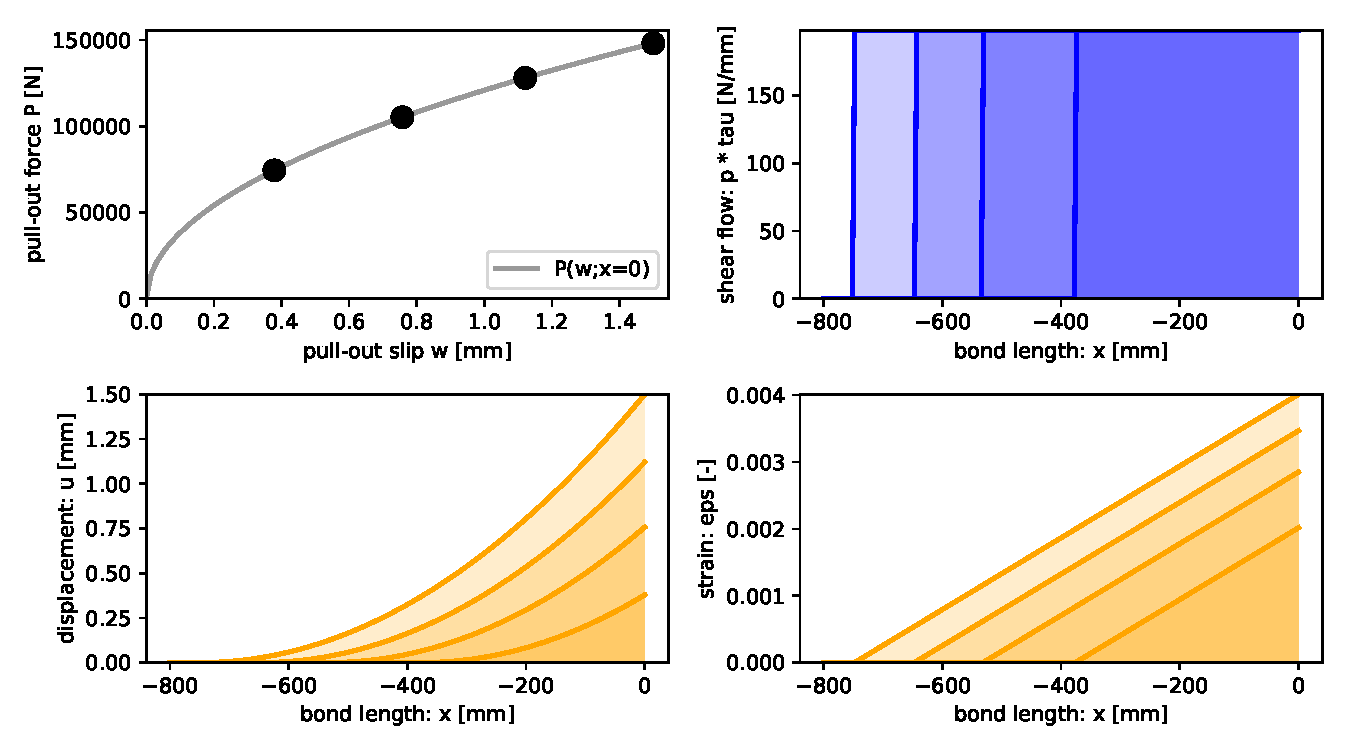
\includegraphics[width=0.95\textwidth]{examples/e31_pullout_frictional/fig_frictional_bond.pdf}
    \end{center}
            \end{bmcsex}
\end{document}
    